\setcounter{page}{2}

\addchap{Цели работы}

Целью работы является освоение принципов эффективного ипользования подсистемы современных универскальных ЭВМ, обеспечивающих хранение и своевременную выдачу команд и данных в центральное процессорное устройство. Работа проводится с использованием программы для сбора и анализа производительности PCLAB.

\chapter{Задание №1}

В этом задании прошло ознакомление с возможностями программы PCLAB. Изучена информация вкладки "Идентификация процесса". Процесс сбора и анализа экспериментальных данных в PCLAB основан на процедуре профилировки критического кода (в измерении времени его обработки центральным процессорным устройством). При запуске программы доступен следующий интерфейс (рис. 1.1):

\begin{figure}[H]
	\begin{center}
		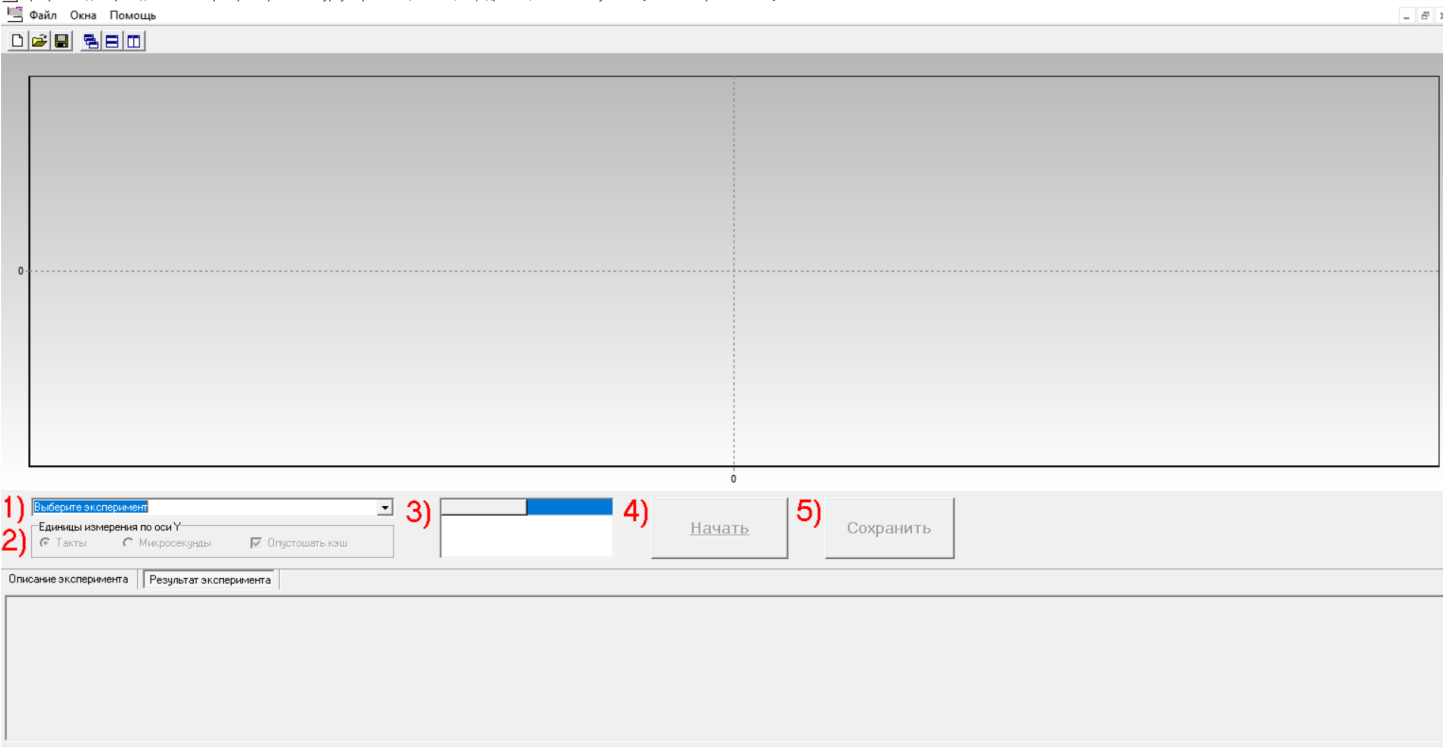
\includegraphics[scale=0.5]{assets/task1.png}
	\end{center}
	\caption{Окно эксперимента}
\end{figure}

В верхней части экрана можно будет увидет зависимость, полученную путем проведения эксперимента. Составляющие интерфейса:
\begin{enumerate}
	\item название эксперимента;
	\item выбор единиц измерения эксперимента;
	\item параметры эксперимента;
	\item старт проведения эксперимента;
	\item сохранение результатов эксперимента.
\end{enumerate}

\chapter{Задание №2}

Благодаря информации со вкладки "Идентификация процесса" были установлены параметры система:
\begin{itemize}
	\item размер линейки кэш-памяти верхнего уровня - 128 Б;
	\item объем физической памяти - 2 ГБ.
\end{itemize}

\chapter{Задание №3}

Результаты эксперимента на рис. 3.1.

\begin{figure}[H]
	\begin{center}
		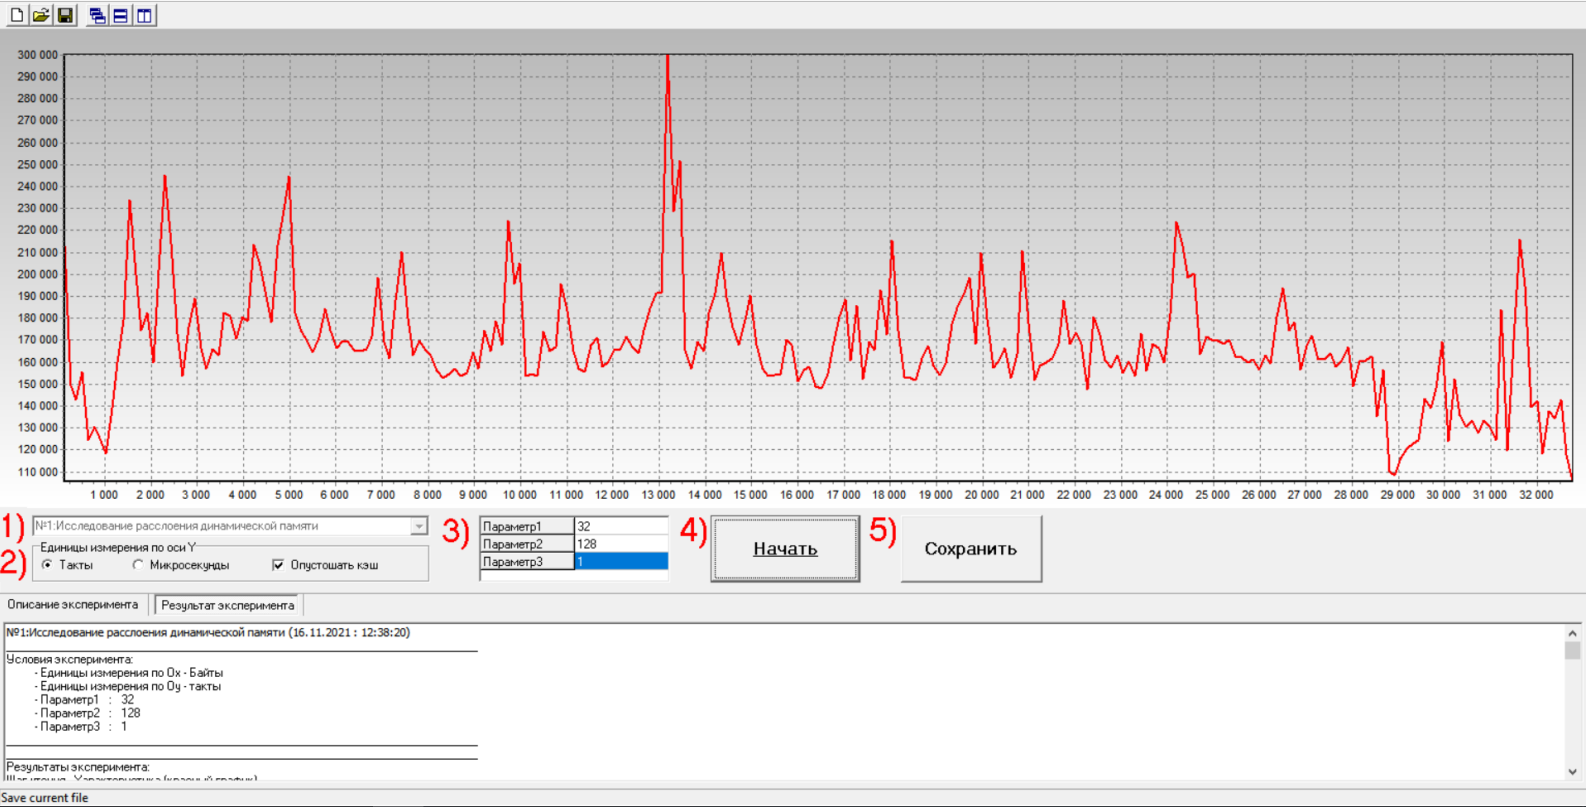
\includegraphics[scale=0.5]{assets/task3.png}
	\end{center}
	\caption{Исследование расслоения динамической памяти}
\end{figure}

До точки T2 = 2048 б наблюдается рост графика, связанный с тем, что при росте шага чтения требуется открытие большего числа страниц. При этом в одном банке памяти может находиться одна и та же открытая страница. Точка T2 - расстояние между началами дух последовательных страница памяти одного банка. Тогда размер страницы памяти можно найти, разделив шаг T2 на число банков.

Точка T1 = 128 б представляет собой точку локального максимума. Эта точка соответствует размеру одного набора. При этом постоянно происходит обращение к одному и тому же банку, то есть не происходит чередование банков памяти. По ее значению этого шага легко можно определить число банков памяти. Для этого размер набора надо разделить на размер линейки Б = T1 / П = 128 б / 128 б = 1.

Размер одной страницы памяти PC = T2 / Б = 2048 б / 1 = 2048 б.

Число страниц физической оперативной памяти C = O / (PC * Б * П) = 2147482648 / (2048 * 1 * 128) = 8192 шт.

Поскольку память состоит из определенного количества банков, наилучшим способом обращения к ней будет обращение к последовательным элементам соседних банков, худшим - обращение к следующей строке одного и того же банка.

\chapter{Задание №4}

Результаты эксперимента представлены на рис. 4.1.

\begin{figure}[H]
	\begin{center}
		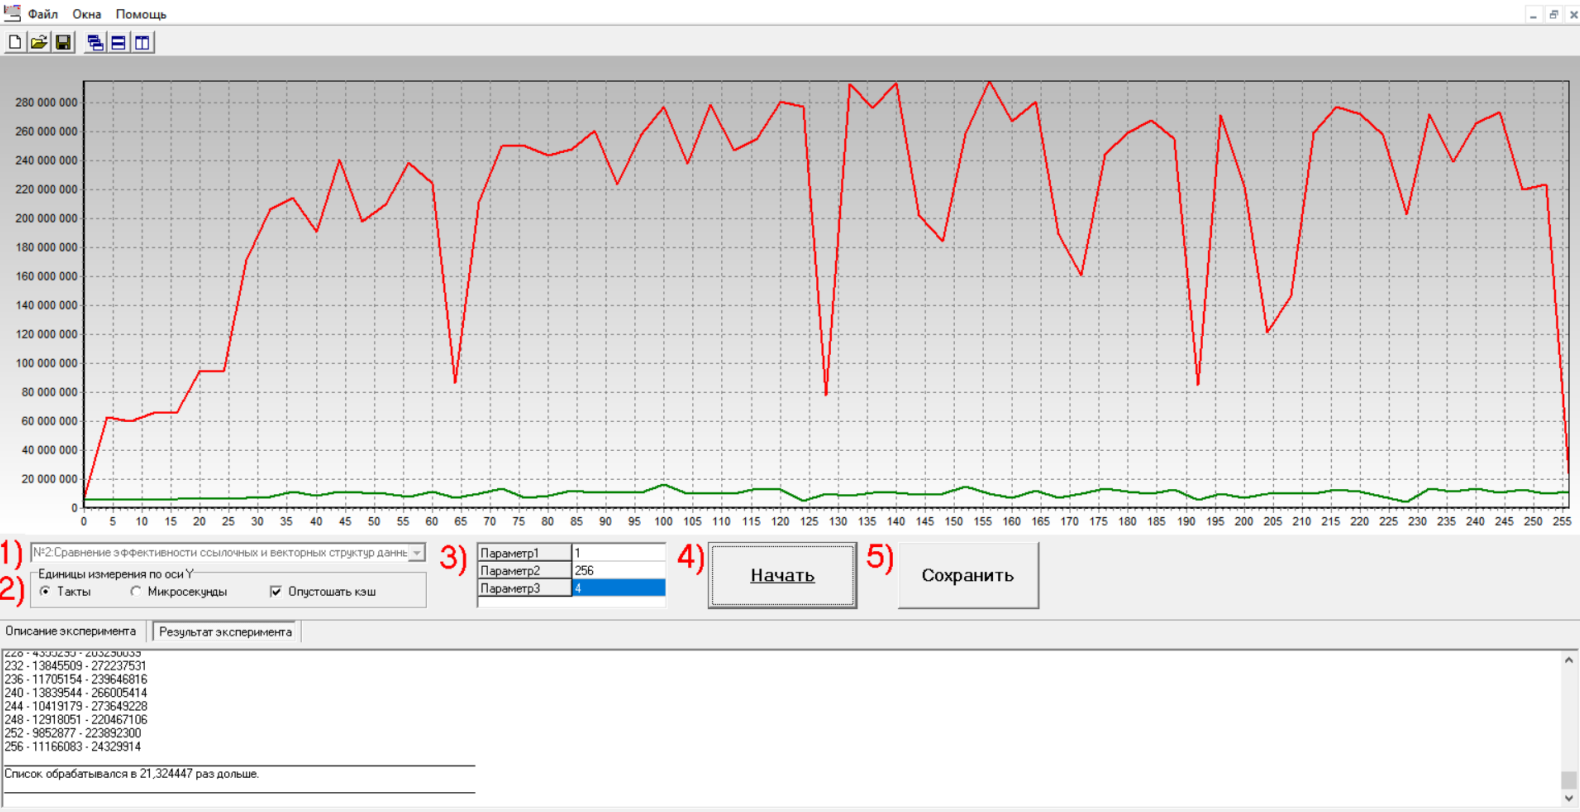
\includegraphics[scale=0.5]{assets/task4.png}
	\end{center}
	\caption{Сравнение эффективности ссылочных и векторных структур данных}
\end{figure}

По результатам эксперимента можно сказать, что список (зависимые данные) орабатываются в среднем в 21.3 раз дольше, чем массив (независимые данные). Можно сделать вывод, что по возможности лучше использовать массив, а не список. При обработке списков адрес следующего элемента станет известен лишь после обращения к текущему, таким образом предвыборка в кэш не производится. При работе с массивами же предвыборка производится, и обработка предзагруженных в кэш и последовательно расположенных в памяти происходит гораздо быстрее.

\chapter{Задание №5}

Результаты эксперимента представлены на рис. 5.1.

\begin{figure}[H]
	\begin{center}
		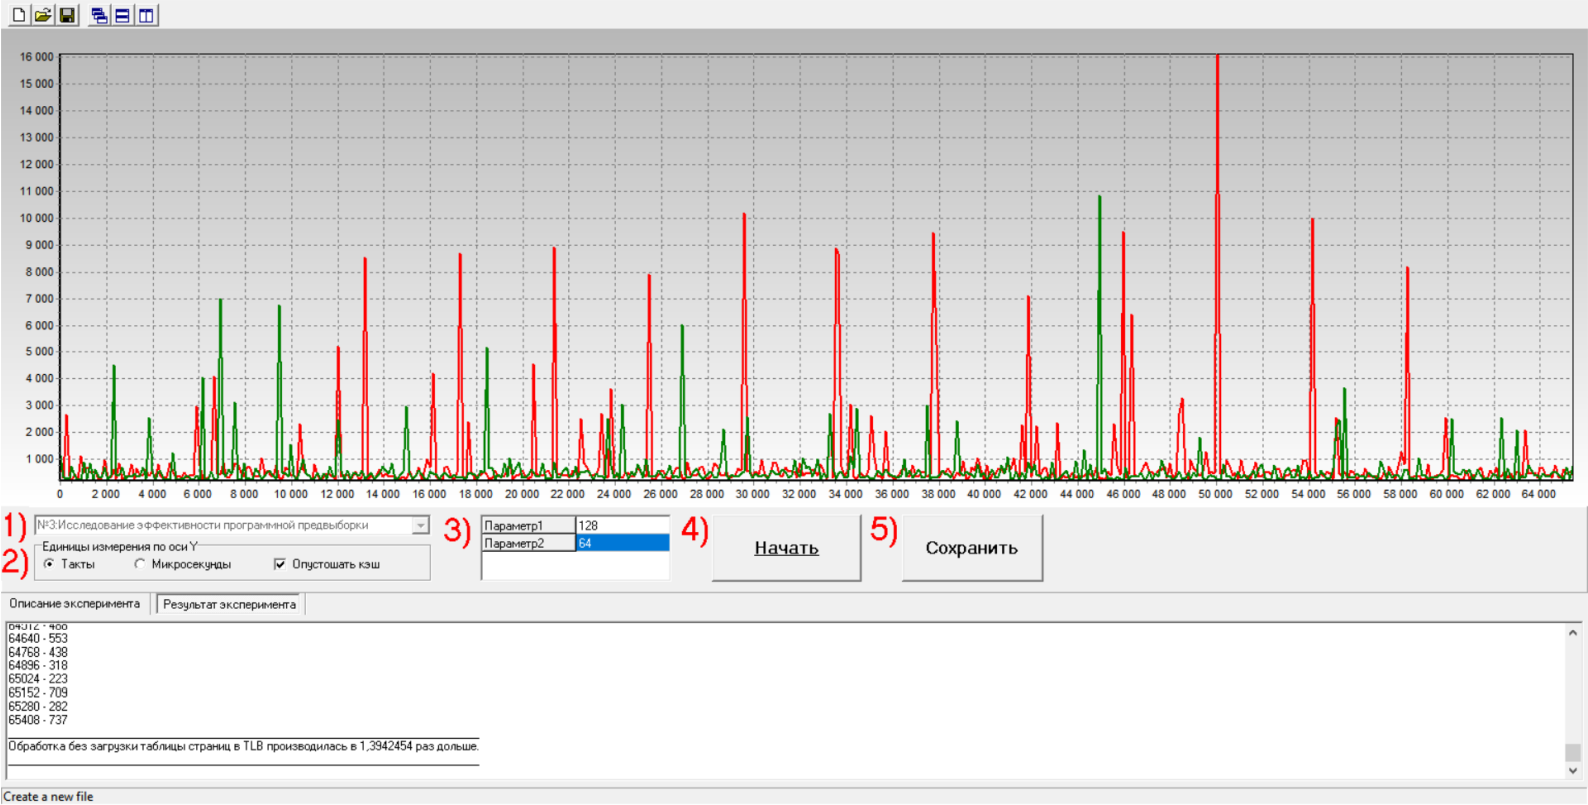
\includegraphics[scale=0.5]{assets/task5.png}
	\end{center}
	\caption{Исследование эффективности программной выборки}
\end{figure}

Обработка без загрузки таблицы страниц в TLB производилась в 1.3942 раз дольше. При обработке больших объемов данных происходит открытие большого числа страниц физической памяти. Возникает необходимость преобразования логических адресов в физические на основании хранимых в TLB процессора данных. Если в TLB процессора отсутствует необходимая информация, то приходится обращаться к оперативной памяти дважды, что приводит к потере производительности. Пики на красном графике соответствуют ситуации, когда инфморация о искомой страице в TLB отсутствовала. Использование прдвыборки позволяет предварительно загрузить данные в TLB, что в ряде случаев повышает производительность.

\chapter{Задание №6}

Результаты эксперимента представлены на рис. 6.1.

\begin{figure}[H]
	\begin{center}
		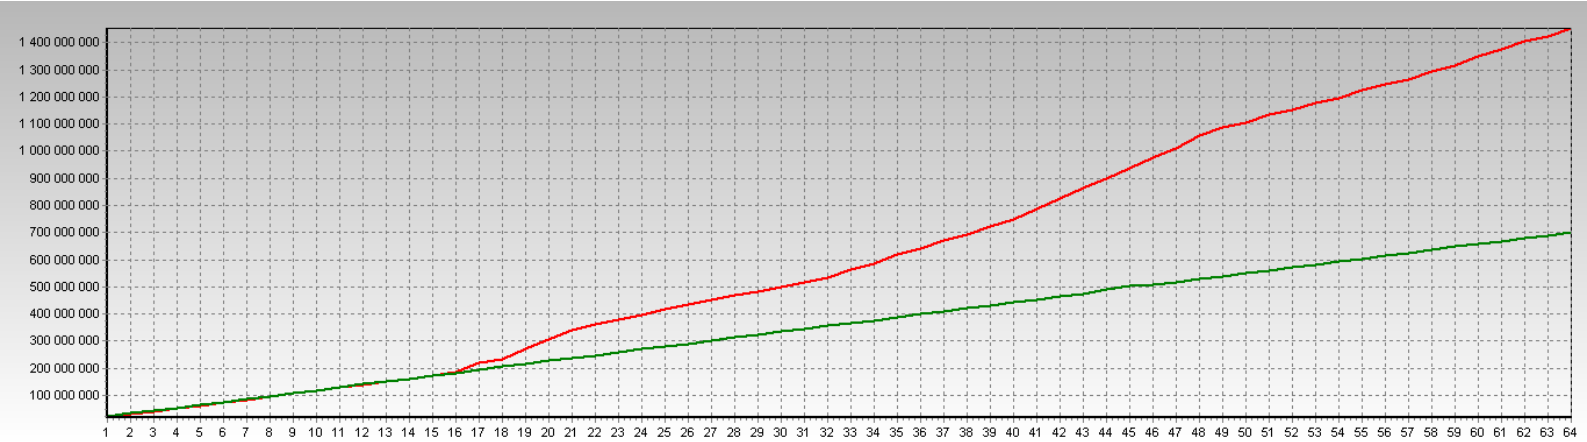
\includegraphics[scale=0.5]{assets/task6.png}
	\end{center}
	\caption{Исследование способов эффективного чтения оперативной памяти}
\end{figure}

Неоптимизировання структура обрабатывалась в 1.3291 раз дольше. При выборке из оперативной памяти происходит получение одной линейкию При этом объеме востребованных данных при программировании на языках высокого уровня зачастую меньше размера линейки. Оптимизация структур данных позволяет передавать в одном пакете только востребованные данные. Это позволяет снизить колиечство кэш-промахов и повышает производительность системы до 2-х раз.

\chapter{Задание №7}

Результаты эксперимента представлены на рис. 7.1.

\begin{figure}[H]
	\begin{center}
		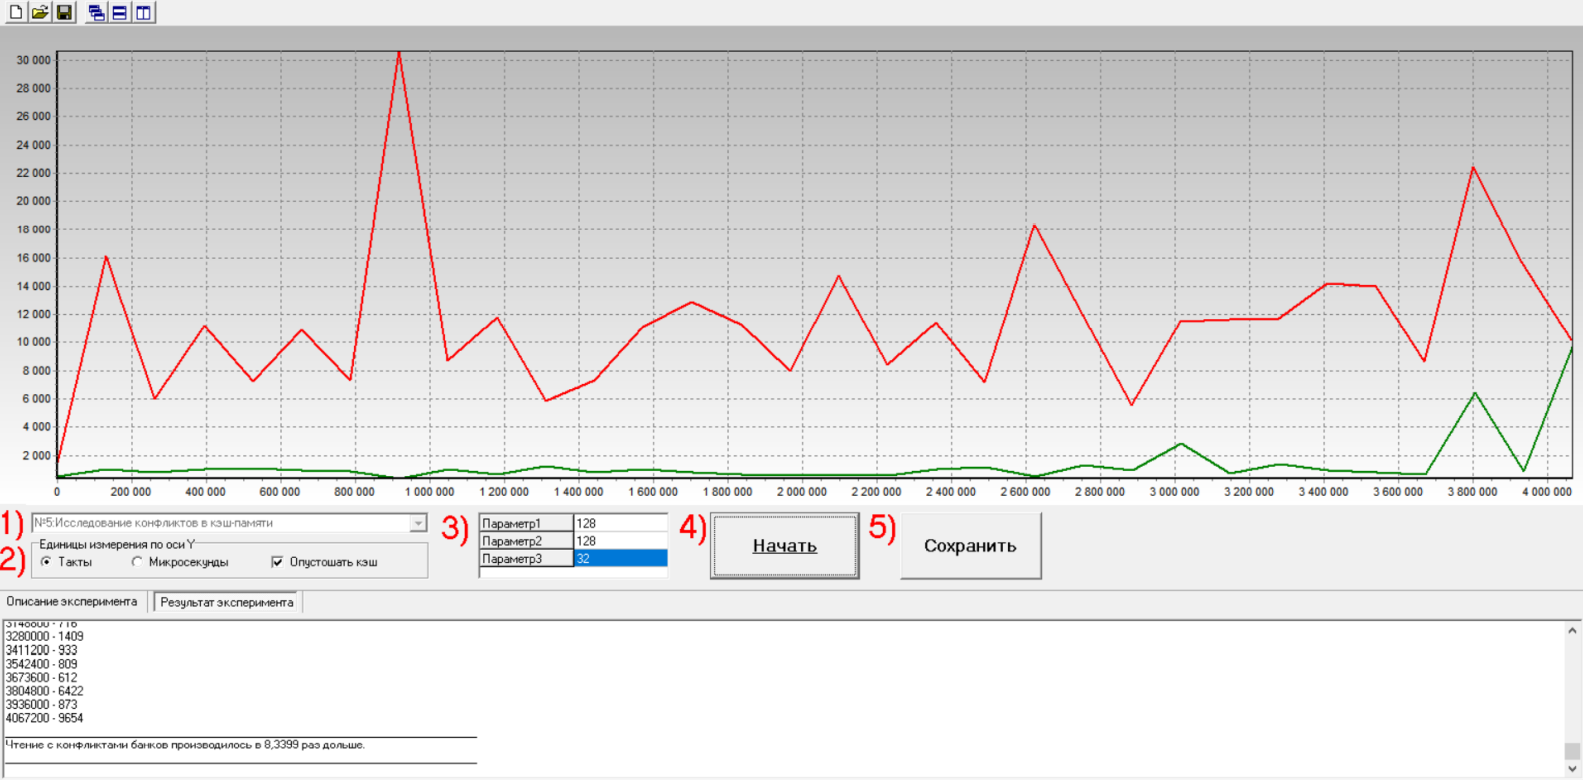
\includegraphics[scale=0.5]{assets/task7.png}
	\end{center}
	\caption{Исследование конфликтов в кэш-памяти}
\end{figure}

Чтение с конфликатми банков производилось в 8.3399 раз дольше. Конфликты в кэш-памяти возникают в случае чтения данных с шагом, кратным размеру банка памяти. В этом случае задействованным будет только один банк памяти и степень ассоциативности памяти "снижается" до 1. При этом наблюдается постоянное вытеснение данных из кэш-памяти и больший её объём остается незадействованным.

\chapter{Задание №8}

Результаты эксперимента представлены на рис. 6.1.

\begin{figure}[H]
	\begin{center}
		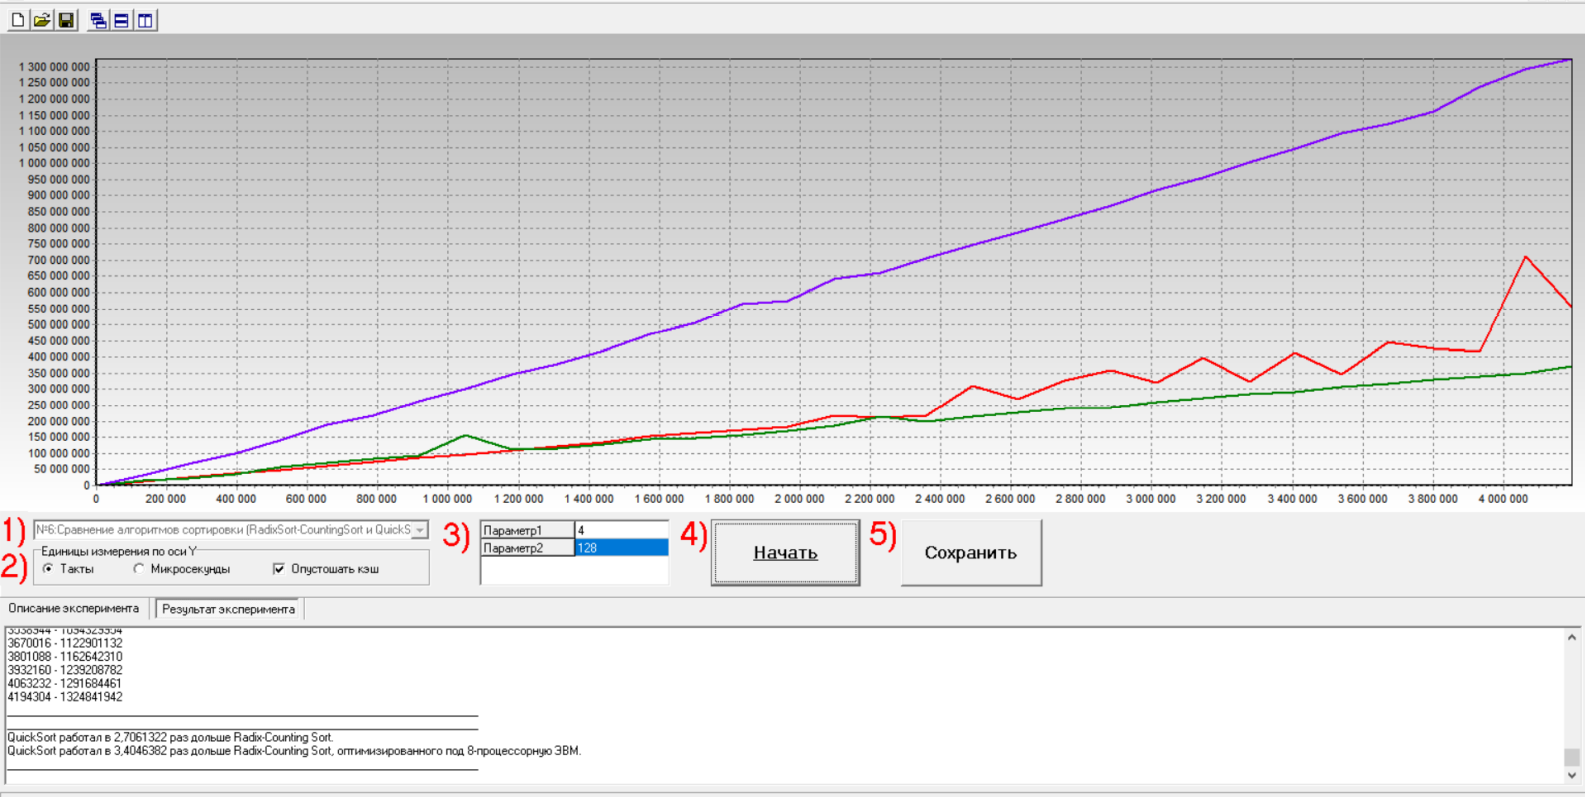
\includegraphics[scale=0.5]{assets/task8.png}
	\end{center}
	\caption{Исследование алгоритмов сортировки}
\end{figure}

QuickSort работал в 2.7061 раз дольше Radix-Counting Sort. QuickSort работал в 3.4046 раз дольше Radix-Counting Sort, оптимизированного под 8-процессорную ЭВМ. За счет разной логики работы различные алгоритмы сортировки по-разному используют физическую память, отчего сильно разнится время доступа к ней и время работы соответственно. Так, QuickSort использует попарные сравнения, отчего увеличивается число обращений к массиву данных, а следовательно и к памяти, в связи с чем увеличивается общее время выполнения сортировки. В Radix-Counting Sort сортировка происходит по-другому, отчего этой подобной проблемы не возникает, что снижает вычислительную сложность. Распараллеливание повышает производительноть и без того быстрого алгоритма.

\addchap{Выводы}

В ходе лабораторной работы были освоены принципы эффективного ипользования подсистемы памяти современных универсальных ЭВМ, обеспечивающей хранение и своевременную выдачу команд и данных в центральное процессорное устройство. С помощью PCLAB был проведен ряд экспериментов на сравнение скорости обращения к блокам данных. Производительность обращения к памяти можно увелиичить за счет использования предвыборки, упорядочивания расположения данных, дабы избежать непредугадываемые обращения к памяти, а также использование структур данных, позволяющих осуществлять предзагрузку данных в кэш-память, параллельную обработку данных.